%%%%%%%%%%%%%%%%%%%%%%%%%%%%%%%%%%%%%%%%%%%%%%%%%%%%%%%%%%%%%%%%%%%%%%%%%%%%%%%%
%% Plantilla de memoria en LaTeX para la EIF - Universidad Rey Juan Carlos
%%
%% Por Gregorio Robles <grex arroba gsyc.urjc.es>
%%     Grupo de Sistemas y Comunicaciones
%%     Escuela de Ingeniería de Fuenlabrada
%%     Universidad Rey Juan Carlos
%% (muchas ideas tomadas de Internet, colegas del GSyC, antiguos alumnos...
%%  etc. Muchas gracias a todos)
%%
%% La última versión de esta plantilla está siempre disponible en:
%%     https://github.com/gregoriorobles/plantilla-memoria
%%
%% Para obtener PDF, ejecuta en la shell:
%%   make
%% (las imágenes deben ir en PNG o JPG)

%%%%%%%%%%%%%%%%%%%%%%%%%%%%%%%%%%%%%%%%%%%%%%%%%%%%%%%%%%%%%%%%%%%%%%%%%%%%%%%%

\documentclass[a4paper, 12pt]{book}
%\usepackage[T1]{fontenc}

\usepackage[a4paper, left=2.5cm, right=2.5cm, top=3cm, bottom=3cm]{geometry}
\usepackage{times}
\usepackage[utf8]{inputenc}
\usepackage[spanish]{babel} % Comenta esta línea si tu memoria es en inglés
\usepackage{url}
%\usepackage[dvipdfm]{graphicx}
\usepackage{graphicx}
\usepackage{float}  %% H para posicionar figuras
\usepackage[nottoc, notlot, notlof, notindex]{tocbibind} %% Opciones de índice
\usepackage{latexsym}  %% Logo LaTeX

\title{Memoria del Proyecto}
\author{Nombre del autor}

\renewcommand{\baselinestretch}{1.5}  %% Interlineado

\begin{document}

\renewcommand{\refname}{Bibliografía}  %% Renombrando
\renewcommand{\appendixname}{Apéndice}


%%%%%%%%%%%%%%%%%%%%%%%%%%%%%%%%%%%%%%%%%%%%%%%%%%%%%%%%%%%%%%%%%%%%%%%%%%%%%%%%
% PORTADA

\begin{titlepage}
\begin{center}
\includegraphics[scale=0.6]{img/URJ_logo_Color_POS.png}

\vspace{1.75cm}

\LARGE
ESCUELA DE INGENIERÍA DE FUENLABRADA
\vspace{1cm}

\LARGE
INGENIERÍA EN SISTEMAS AUDIOVISUALES Y MULTIMEDIA

\vspace{1cm}
\LARGE
\textbf{TRABAJO FIN DE GRADO}

\vspace{2cm}

\Large
PLATAFORMA WEB PARA PROYECTOS DE ARQUITECTURA

\vspace{2cm}

\large
Autor : Bayas Pancho, Karol Joseth \\
Tutor : Robles Martínez, Gregorio\\
Cotutor: De Jorge Huertas, Virginia 
\vspace{1cm}

\large
Curso académico 202X/202X

\end{center}
\end{titlepage}

\newpage
\mbox{}
\thispagestyle{empty} % para que no se numere esta pagina



%%%%%%%%%%%%%%%%%%%%%%%%%%%%%%%%%%%%%%%%%%%%%%%%%%%%%%%%%%%%%%%%%%%%%%%%%%%%%%%%
%%%% Para firmar
\clearpage
\pagenumbering{gobble}
\chapter*{}

\vspace{-4cm}
\begin{center}
\LARGE
\textbf{Trabajo Fin de Grado}

\vspace{1cm}
\large
Plataforma WEB para Proyectos de Arquitectura

\vspace{1cm}
\large
\textbf{Autor :} Bayas Pancho, Karol Joseth \\
\textbf{Tutor :} Robles Martínez, Gregorio

\end{center}

\vspace{1cm}
La defensa del presente Proyecto Fin de Carrera se realizó el día \qquad$\;\,$ de \qquad\qquad\qquad\qquad \newline de 2024, siendo calificada por el siguiente tribunal:


\vspace{0.5cm}
\textbf{Presidente:}

\vspace{1.2cm}
\textbf{Secretario:}

\vspace{1.2cm}
\textbf{Vocal:}


\vspace{1.2cm}
y habiendo obtenido la siguiente calificación:

\vspace{1cm}
\textbf{Calificación:}


\vspace{1cm}
\begin{flushright}
Fuenlabrada, a \qquad$\;\,$ de \qquad\qquad\qquad\qquad de 202X
\end{flushright}

%%%%%%%%%%%%%%%%%%%%%%%%%%%%%%%%%%%%%%%%%%%%%%%%%%%%%%%%%%%%%%%%%%%%%%%%%%%%%%%%
%%%% Dedicatoria

\chapter*{}
\pagenumbering{Roman} % para comenzar la numeracion de paginas en numeros romanos
\begin{flushright}
\textit{Dedicado a \\
mi familia / mi abuelo / mi abuela}
\end{flushright}

%%%%%%%%%%%%%%%%%%%%%%%%%%%%%%%%%%%%%%%%%%%%%%%%%%%%%%%%%%%%%%%%%%%%%%%%%%%%%%%%
%%%% Agradecimientos

\chapter*{Agradecimientos}
%\addcontentsline{toc}{chapter}{Agradecimientos} % si queremos que aparezca en el índice
\markboth{AGRADECIMIENTOS}{AGRADECIMIENTOS} % encabezado 

Con la finalizacion de este proyecto doy por finalizada mi etapa universitaris por lo que 
antetodo me gustaria presentar la gratitud que siento hacia los profesores de la ETSI. A 
lo largo de estos años, su orientación y sabiduría me han guiado en mi camino académico. 
En particular, quiero expresar mi sincero agradecimiento a Gregorio Robles, quien no solo nos 
introdujo en el mundo del desarrollo web, sino que también creyó en mí para la realización de 
este proyecto. Su constante disponibilidad para orientarme y su apoyo inquebrantable han sido invaluables.

También deseo expresar mi amor y gratitud hacia mi familia; a mis padres y hermanos que siempre han estado a mi lado. 
Su apoyo incondicional y constante ha sido mi roca en los momentos de dificultad. Sus palabras de aliento siempre me 
impulsaron a seguir adelante incluso cuando el camino era difícil. Su amor y apoyo han sido la columna vertebral de 
todos mis logros y por eso, estoy eternamente agradecido. 

Y a todos los que de alguna manera han contribuido a este trabajo, muchas gracias. Cada palabra de aliento, cada 
gesto de apoyo, ha sido fundamental para llegar hasta aquí. Este logro es tan suyo como mío.


%%%%%%%%%%%%%%%%%%%%%%%%%%%%%%%%%%%%%%%%%%%%%%%%%%%%%%%%%%%%%%%%%%%%%%%%%%%%%%%%
%%%% Resumen

\chapter*{Resumen}
%\addcontentsline{toc}{chapter}{Resumen} % si queremos que aparezca en el índice
\markboth{RESUMEN}{RESUMEN} % encabezado

Este proyecto es la culminación de mi grado en Ingeniería en Sistemas Audiovisuales y Multimedia, y es la construcción de una 
plataforma web diseñada especialmente para los amantes de la arquitectura. 

Usando el framework Flask de Python, la plataforma busca potenciar la colaboración y comunicación entre los estudiantes y profesores 
de arquitectura. La idea es proporcionar un espacio en el que los usuarios, ya sean estudiantes o profesores, puedan interactuar y 
compartir información relevante. Así, una vez estás registrado, puedes realizar varias tareas, como añadir eventos o libros, compartir 
enlaces interesantes y mucho más. 

La plataforma tiene a un administrador el cual tiene acceso a todas las partes del sistema y puede manejar la base de datos. 
De esta manera, si algo va mal o si necesitamos modificar algo en la base de datos, el administrador puede hacerlo sin problemas.

Además la plataforma permite la carga y gestión de archivos, incluyendo imágenes, videos y documentos PDF. Estos 
archivos están a menudo vinculados a los libros de arquitectura presentes en la plataforma, proporcionando así una valiosa fuente de 
conocimiento e inspiración para cualquiera que esté interesado en la arquitectura. 

Esta plataforma esta pensada para ser accesible desde cualquier navegador, por lo que puedes acceder a ella en tu móvil, tableta o 
cualquier otro dispositivo. 

Cuenta además con diferentes tipos de usuarios por lo que si eres un alumno o un profesor, la plataforma te ofrece diferentes funcionalidades. 
Esto se hace para asegurar que cada usuario tenga una experiencia adaptada a sus necesidades y pueda aprovechar al máximo la plataforma.

En resumen, este proyecto no es solo una plataforma que facilita la colaboración entre alumnos y profesores de arquitectura. Es también 
una biblioteca virtual de conocimiento arquitectónico y una potente herramienta para mejorar la experiencia educativa en el campo de la 
arquitectura.

%%%%%%%%%%%%%%%%%%%%%%%%%%%%%%%%%%%%%%%%%%%%%%%%%%%%%%%%%%%%%%%%%%%%%%%%%%%%%%%%
%%%% Resumen en inglés

\chapter*{Summary}
%\addcontentsline{toc}{chapter}{Summary} % si queremos que aparezca en el índice
\markboth{SUMMARY}{SUMMARY} % encabezado

This project represents the culmination of my degree in Audiovisual and Multimedia Systems Engineering, 
which culminated in the creation of a web platform specifically designed for architecture enthusiasts.

Using Python's Flask framework, the platform aims to enhance collaboration and communication among students 
and professors in the field of architecture. The goal is to provide a space where users, both students and professors, 
can interact and share relevant information. Once you are registered, you can engage in various tasks such as adding events 
or books, sharing interesting links, and much more.

The platform has an administrator who has access to all parts of the system and can manage the database. Therefore, if 
something goes wrong or if we need to modify something in the database, the administrator can take charge without any issues.

Moreover, the platform allows users to upload and manage files, including images, videos, and PDF documents. These files are 
often linked to architecture books present on the platform, providing a valuable source of knowledge and inspiration for anyone 
interested in architecture.

This platform is designed to be accessible from any browser, so you can access it from your mobile phone, tablet, or any other device.

In addition, the platform offers different functionalities based on whether you are a student or a professor. This is accomplished 
in order to ensure that each user has an experience tailored to their needs and can make the most out of the platform.

In summary, this project is not only about a platform facilitating collaboration between students and teachers of architecture. It's 
also a virtual library of architectural knowledge and a powerful tool for enhancing the educational experience in the field of 
architecture.

%%%%%%%%%%%%%%%%%%%%%%%%%%%%%%%%%%%%%%%%%%%%%%%%%%%%%%%%%%%%%%%%%%%%%%%%%%%%%%%%
%%%%%%%%%%%%%%%%%%%%%%%%%%%%%%%%%%%%%%%%%%%%%%%%%%%%%%%%%%%%%%%%%%%%%%%%%%%%%%%%
% ÍNDICES %
%%%%%%%%%%%%%%%%%%%%%%%%%%%%%%%%%%%%%%%%%%%%%%%%%%%%%%%%%%%%%%%%%%%%%%%%%%%%%%%%

% Las buenas noticias es que los índices se generan automáticamente.
% Lo único que tienes que hacer es elegir cuáles quieren que se generen,
% y comentar/descomentar esa instrucción de LaTeX.

%%%% Índice de contenidos
\tableofcontents 
%%%% Índice de figuras
\cleardoublepage
%\addcontentsline{toc}{chapter}{Lista de figuras} % para que aparezca en el indice de contenidos
\listoffigures % indice de figuras
%%%% Índice de tablas
%\cleardoublepage
%\addcontentsline{toc}{chapter}{Lista de tablas} % para que aparezca en el indice de contenidos
%\listoftables % indice de tablas


%%%%%%%%%%%%%%%%%%%%%%%%%%%%%%%%%%%%%%%%%%%%%%%%%%%%%%%%%%%%%%%%%%%%%%%%%%%%%%%%
%%%%%%%%%%%%%%%%%%%%%%%%%%%%%%%%%%%%%%%%%%%%%%%%%%%%%%%%%%%%%%%%%%%%%%%%%%%%%%%%
% INTRODUCCIÓN %
%%%%%%%%%%%%%%%%%%%%%%%%%%%%%%%%%%%%%%%%%%%%%%%%%%%%%%%%%%%%%%%%%%%%%%%%%%%%%%%%

\cleardoublepage
\chapter{Introducción}
\label{sec:intro} % etiqueta para poder referenciar luego en el texto con ~\ref{sec:intro}
\pagenumbering{arabic} % para empezar la numeración de página con números

En el terreno educativo de la arquitectura, la colaboración eficiente y la comunicación fluida se están convirtiendo en elementos 
indispensables. Esta necesidad ha quedado plasmada en el proyecto que les presento hoy: una plataforma web construida con la finalidad 
de potenciar la interacción entre estudiantes y profesores del mundo arquitectónico.

La plataforma está diseñada para el intercambio de información relevante y facilita la comunicación en torno a los eventos en curso a 
lo largo del calendario académico.

Promoviendo activamente la dinámica académica, este proyecto no es sólo una recopilación del conocimiento técnicos adquiridos durante 
el grado, sino que también representa un proyecto para mejorar la educación arquitectónica. 

\section{Motivación}
\label{sec:seccion}


En el trasfondo de la educación arquitectónica, me impulsa la firme convicción de que la tecnología puede desempeñar un papel transformador al mejorar la colaboración y la comunicación entre estudiantes y profesores. Inspirado por mis tutores Virginia y Gregorio en el deseo de superar las barreras existentes en la interacción educativa, he decidido emprender el desarrollo de esta plataforma web.

La motivación central detrás de esta iniciativa es la necesidad de proporcionar a la comunidad educativa de arquitectura una herramienta digital que simplifique y enriquezca su experiencia de aprendizaje. Observando las limitaciones en la comunicación y el intercambio de información, he visualizado esta plataforma como un espacio virtual donde la colaboración se vuelve intuitiva y donde la información relevante fluye de manera efectiva.

Con el objetivo de fomentar la participación activa, la plataforma busca ir más allá de ser simplemente un repositorio de datos. Pretende ser un medio dinámico donde los estudiantes pueden compartir ideas, los profesores pueden proporcionar orientación y todos pueden estar al tanto de los eventos educativos cruciales. La creación de esta plataforma no solo es un ejercicio técnico, sino una contribución tangible a la mejora de la calidad educativa en el ámbito de la arquitectura.

Creo firmemente que, al proporcionar un entorno digital eficiente y fácil de usar, esta plataforma puede marcar la diferencia al facilitar la colaboración, fomentar la comunicación y, en última instancia, elevar el estándar de la educación arquitectónica. Esta motivación arraigada en la mejora continua y la innovación tecnológica impulsa mi dedicación a la creación de esta herramienta que aspira a enriquecer la experiencia educativa para estudiantes y profesores por igual.
\section{Objetivos e hipótesis de investigación}
\label{sec:seccion}

\subsection{Objetivos de Investigación}
\label{subsec:Objetivos de Investigación}

\begin{itemize}
  \item Facilitar la Colaboración: Crear un entorno digital que promueva la colaboración entre estudiantes y profesores de arquitectura, facilitando el intercambio de información y recursos educativos.
  \item Centralizar Recursos: Desarrollar una plataforma que sirva como repositorio central para libros, archivos y otros recursos relacionados con la arquitectura, mejorando el acceso y la gestión de la información educativa.
  \item Mejorar la Comunicación: Implementar herramientas de comunicación efectiva, como la organización de eventos y foros, para fomentar la interacción activa y el intercambio de ideas entre los usuarios.
  \item Optimizar la Experiencia del Usuario: Diseñar una interfaz intuitiva y fácil de usar que se adapte a las necesidades específicas de los estudiantes y profesores de arquitectura, mejorando la experiencia de navegación y participación.
\end{itemize}

\subsection{Hipótesis de Investigación}
\label{subsec:Hipótesis de Investigación}

\begin{itemize}
  \item Mayor Colaboración: Se espera que la implementación de la plataforma web aumente la colaboración entre estudiantes y profesores, proporcionando un espacio digital propicio para compartir conocimientos y experiencias.
  \item Eficiencia en la Gestión de Recursos: La centralización de recursos, como libros y archivos, en la plataforma resultará en una gestión más eficiente y accesible de los materiales educativos, beneficiando tanto a estudiantes como a profesores.
  \item Mejora en la Comunicación: La introducción de herramientas de comunicación, como eventos y foros, contribuirá a una comunicación más efectiva entre los usuarios, fomentando la participación activa y la discusión de temas relevantes.
  \item Aumento de la Participación: La optimización de la experiencia del usuario en la plataforma generará un aumento en la participación, ya que los usuarios encontrarán la interfaz intuitiva y amigable, facilitando su interacción con la plataforma.
\end{itemize}



\section{Estructura de la memoria}
\label{sec:seccion}

A continuación, se presenta una descripción de la estructura de la memoria, 
detallando el contenido de cada uno de los capítulos para proporcionar 
una guía organizada del trabajo de fin de grado:

\begin{itemize}
  \item \textbf{Capítulo 1:} Introducción \\
  En este capítulo, se presenta el contexto del trabajo, se define el problema de 
  investigación y se destacan los objetivos del estudio. Además, se ofrece una breve 
  descripción de la metodología utilizada y se justifica la relevancia del tema.
  \item \textbf{Capítulo 2:} Objetivos del Proyecto \\
  En este capítulo se proporciona información detallada sobre el diseño, las 
  características y los usos de cada una de las tecnologías usadas en el proyecto. 

  \item \textbf{Capítulo 3:} Tecnologías Utilizadas \\
  En este capítulo se proporciona información detallada sobre el diseño, las 
  características y los usos de cada una de las tecnologías usadas en el proyecto.

  \item \textbf{Capítulo 4:} Funcionamiento de la Aplicación \\
  En este capítulo, se entra en detalle en el funcionamiento de la aplicación.

  \item \textbf{Capítulo 5:} Experimentos y Pruebas \\
  Se presentan los diferentes experimentos realizados y se prueba el correcto funcionamiento de la aplicación.

  \item \textbf{Capítulo 6:} Resultados Obtenidos \\
  En este capítulo, se explican los resultados obtenidos al poner a prueba varios aspectos de la aplicación.

  \item \textbf{Capítulo 7:} Conclusiones \\
  Se indican los resultados conseguidos y la solución a los objetivos no conseguidos.
\end{itemize}


%%%%%%%%%%%%%%%%%%%%%%%%%%%%%%%%%%%%%%%%%%%%%%%%%%%%%%%%%%%%%%%%%%%%%%%%%%%%%%%%
%%%%%%%%%%%%%%%%%%%%%%%%%%%%%%%%%%%%%%%%%%%%%%%%%%%%%%%%%%%%%%%%%%%%%%%%%%%%%%%%
% OBJETIVOS %
%%%%%%%%%%%%%%%%%%%%%%%%%%%%%%%%%%%%%%%%%%%%%%%%%%%%%%%%%%%%%%%%%%%%%%%%%%%%%%%%

\cleardoublepage % empezamos en página impar
\chapter{Objetivos} % título del capítulo (se muestra)
\label{chap:objetivos} % identificador del capítulo (no se muestra, es para poder referenciarlo)

\section{Objetivo general} % título de sección (se muestra)
\label{sec:objetivo-general} % identificador de sección (no se muestra, es para poder referenciarla)
El propósito de este proyecto es crear un sistema de administración destinado a gestionar libros, documentos y eventos. 
Su objetivo principal es mejorar la experiencia de los usuarios al facilitar el acceso a la información a través de una 
interfaz intuitiva. Para garantizar la seguridad de la plataforma, se implementarán funcionalidades como inicio de sesión 
y restablecimiento de contraseña.

En esta plataforma, nos centramos en la interacción de los usuarios para la gestión de eventos y la administración de libros. 
También hemos integrado herramientas administrativas que facilitarán a los usuarios interactuar de manera eficiente y efectiva. 
Queremos que la experiencia sea lo más amigable posible para todos los que utilicen este sistema.
\section{Objetivos específicos}
\label{sec:objetivos-especificos}
\begin{enumerate}
  \item \textbf{Desarrollar vistas de administración:} Crear vistas administrativas para la gestión de libros, eventos y usuarios.
  \item \textbf{Sistema de autenticación:} Desarrollar un sistema de autenticación para permitir el acceso seguro a las funcionalidades administrativas.
  \item \textbf{Diseñar páginas de visualización:} Diseñar páginas de visualización de libros, eventos y comentarios para todos los usuarios.
  \item \textbf{Integrar un sistema de comentarios:} Integrar un sistema de comentarios para permitir a los usuarios expresar sus opiniones sobre los libros.
  \item \textbf{Gestión de eventos:} Implementar la gestión de eventos, permitiendo la visualización y edición de ellos.
  \item \textbf{Administrar libros:} Desarrollar funciones para agregar, editar y eliminar libros ademas de asociarlos con autores.
  \item \textbf{Herramientas administrativas:} Implementar herramientas administrativas para la gestión de usuarios, roles y permisos.
  \item \textbf{Optimizar seguridad:} Mejorar la seguridad de las contraseñas mediante el uso de técnicas seguras de almacenamiento y recuperación.
  \item \textbf{Restricciones de acceso:} Aplicar restricciones de acceso basadas en roles para controlar qué usuarios pueden acceder a determinadas funcionalidades.
  \item \textbf{Integridad de los datos:} Implementar medidas para garantizar la integridad de los datos, evitando inconsistencias y errores en la base de datos.
\end{enumerate}

\section{Planificación temporal}
\label{sec:planificacion-temporal}
La ejecución de este proyecto de Trabajo de Fin de Grado correspondió a un período de ocho meses, desde julio de 2023 hasta febrero de 2024. A continuación, un breve desglose de la planificación temporal del proyecto:

\begin{itemize}
  \item Julio 2023: Mes de presentación del proyecto bajo la mentoría del profesor Gregorio Robles Martínez.  Durante este mes también comencé mis reuniones con Virginia, mi codirectora de Trabajo de Fin de Grado (TFG). Juntos comenzamos a esbozar los elementos básicos que queríamos incorporar en el sitio web.
  \item Agosto 2023: Dediqué este mes a repetidas consultas con Virginia para afinar la visión del proyecto. Se llevó a cabo una exploración exhaustiva de varias páginas web enfocadas en arquitectura para ayudar a infundir ideas innovadoras en nuestra propia plataforma.
  \item Agosto - Octubre 2023: Durante este período, estuve inmerso en la fase de implementación y desarrollo de la plataforma web. Construí páginas dedicadas para usuarios registrados y también para visitantes. En sesiones tutoriales, nos enfocamos en aspectos técnicos como el manejo de permisos de usuarios, la incorporación de un sistema de admisión de usuarios y la funcionalidad de recuperación de contraseñas.
  \item Noviembre - Diciembre 2023: En estos meses, realicé importantes adiciones a la plataforma, integrando un calendario y una sección de libros para enriquecer la experiencia del usuario. Se permitieron los comentarios pero limitados a los usuarios registrados.
  \item Enero - Febrero 2024: Durante los últimos dos meses, la atención se centró en la redacción del informe final del proyecto, junto con la corrección de ciertos detalles en el código según las necesidades identificadas.
\end{itemize}

\begin{figure}
  \centering
  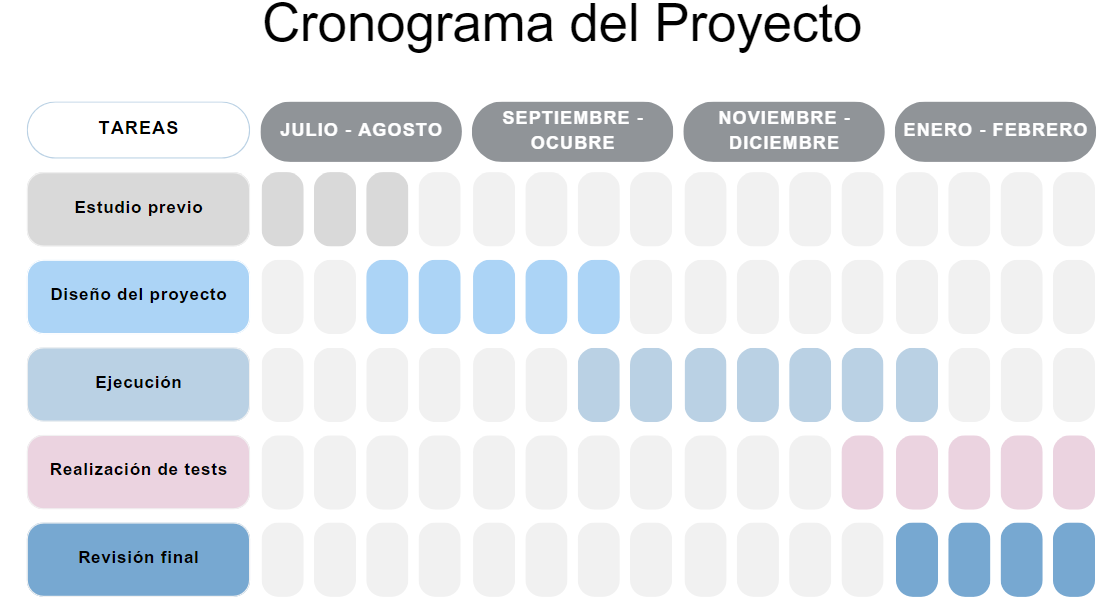
\includegraphics[width=15cm, keepaspectratio]{img/gann.png}
  \caption{Diagrama de Gantt}
  \label{fig:arquitectura}
\end{figure}


%%%%%%%%%%%%%%%%%%%%%%%%%%%%%%%%%%%%%%%%%%%%%%%%%%%%%%%%%%%%%%%%%%%%%%%%%%%%%%%%
%%%%%%%%%%%%%%%%%%%%%%%%%%%%%%%%%%%%%%%%%%%%%%%%%%%%%%%%%%%%%%%%%%%%%%%%%%%%%%%%
% ESTADO DEL ARTE %
%%%%%%%%%%%%%%%%%%%%%%%%%%%%%%%%%%%%%%%%%%%%%%%%%%%%%%%%%%%%%%%%%%%%%%%%%%%%%%%%

\cleardoublepage
\chapter{Estado del arte}
\label{chap:estado}

En este capítulo se mostraran las herramientas y liberías usadas en el Trabajo de Fin de Grado. Esto nos 
dara una visión de las tecnologias utilizadas a lo largo del proyecto.

\section{Tecnologías y Herramientas}
\label{sec:tecnologías y herramientas}

\subsection{Python} 
\label{subsec:Python} Python\footnote{\url{https://www.python.org/}}, desarrollado por Guido van Rossum a finales de los 80 en los Países Bajos, es un lenguaje 
de programación con un enfoque en la legibilidad del código y la productividad del programador. Desde su primera versión en 1991, ha 
experimentado un crecimiento significativo y se ha convertido en uno de los lenguajes más populares y utilizados en la actualidad. Su sintaxis simple, 
clara y precisa facilita la escritura de código limpio, mientras que su extensa gama de bibliotecas estándar acelera el proceso de desarrollo. 
Su adaptabilidad y compatibilidad con diversos paradigmas de programación han permitido su uso en una amplia variedad de aplicaciones, desde el 
desarrollo de software hasta el análisis de datos y machine learning.

\subsection{GitHub} 
\label{subsec:github} GitHub \footnote{\url{https://github.com/}} es un servicio en la nube que aloja un sistema de control de versiones, Git, lo que permite a los 
desarrolladores colaborar en proyectos compartidos manteniendo un seguimiento detallado de su progreso. Funciona como una plataforma web para el 
desarrollo colaborativo de software, facilitando la colaboración y el almacenamiento de proyectos de código abierto o privado. En GitHub, los usuarios 
pueden trabajar juntos en proyectos, compartiendo ideas y soluciones. Su principal ventaja es la posibilidad de trabajar en un proyecto en cualquier 
lugar y momento, ya que se realiza un seguimiento del desarrollo de forma remota. Además, proporciona otras funciones vitales a los desarrolladores, 
como bibliotecas y funciones para la gestión de versiones de software, la gestión de problemas y la revisión de código.

\subsection{PHPMyAdmin}
\label{subsec:phpmyadmin} PHPMyAdmin\footnote{\url{http://localhost/phpmyadmin/}} es una herramienta creada en PHP que facilita la administración de bases de datos 
MySQL a través de una interfaz de usuario en un navegador web. 
Entre sus funciones se incluyen: la creación, modificación y eliminación de bases de datos y tablas; la gestión de campos y el ajuste de privilegios; y la 
capacidad de exportar datos en varios formatos. Esta herramienta multilingüe está disponible bajo la licencia GPL Versión 2. Desde su creación en 1998, 
PHPMyAdmin ha experimentado continuos avances y adaptaciones a las máquinas con servidores web y soporte de PHP y MySQL.

\subsection{JavaScript}
\label{subsec:JavaScript} JavaScript\footnote{\url{https://lenguajejs.com/javascript/}} es un lenguaje de programación de alto nivel, interpretado y orientado a objetos, conocido por su capacidad para ofrecer 
interactividad a las páginas web. Es un lenguaje del lado del cliente, por lo que se ejecuta en el navegador del usuario y puede interactuar con el contenido 
de la página, el Document Object Model (DOM) y otros elementos del navegador. Puede manipular el contenido de la página y responder a eventos del usuario. 
Además, es un lenguaje asincrónico, lo que le permite realizar tareas sin bloquear la ejecución del código. Es esencial para la manipulación del DOM, permitiendo 
agregar, eliminar o modificar elementos dinámicamente. También maneja eventos del usuario, facilita la creación de aplicaciones web interactivas y utiliza 
tecnologías como XMLHttpRequest o la interfaz Fetch para realizar solicitudes asíncronas al servidor. Dispone de diversos frameworks y bibliotecas que facilitan 
el desarrollo de aplicaciones web complejas. Además, sigue las especificaciones definidas por ECMAScript y es pluriparadigmático, admitiendo varios estilos de 
programación.

Docker\footnote{\url{https://www.docker.com/}} es una plataforma de código abierto que permite automatizar el despliegue, la escalabilidad y la operación de 
aplicaciones dentro de contenedores de software. Estos contenedores permiten empaquetar una aplicación junto con todas sus dependencias en una unidad estandarizada 
para el desarrollo de software, lo que facilita su portabilidad entre distintos entornos.

Algunos de los puntos clave de Docker son:

\begin{enumerate}
  \item \textbf{Portabilidad:} Docker permite empaquetar y ejecutar aplicaciones en prácticamente cualquier entorno, lo que facilita la migración de aplicaciones y sistemas.
  \item \textbf{Aislamiento:} Los contenedores de Docker permiten el aislamiento de recursos, lo que garantiza que cada contenedor funcione como una unidad autónoma y que los problemas en un contenedor no afecten a otros.
  \item \textbf{Eficiencia:} Docker es muy eficiente en términos de rendimiento ya que los contenedores que utiliza consumen menos recursos que las máquinas virtuales equivalentes.
  \item \textbf{Escalabilidad:} Docker facilita la escalabilidad de las aplicaciones, ya que permite crear y desplegar contenedores rápidamente y en gran medida.
  \item \textbf{Integración continua y entrega continua (CI/CD):} Docker se integra bien con los sistemas de CI/CD, lo que permite probar las aplicaciones en contenedores en distintas etapas del desarrollo y despliegue de forma automatizada.
  \item \textbf{Descentralización del desarrollo:} Docker ayuda a los equipos de desarrollo a trabajar de manera descentralizada y colaborativa, ya que cualquier miembro del equipo puede crear y desplegar contenedores con su propio trabajo. 
\end{enumerate}

\section{Liberías}
\label{sec:Librerias}

Descripción de las tecnologías utilizadas en el proyecto. 

\subsection{Flask-Login}
\label{subsec:flasklogin} Flask-Login es una extensión de Flask que proporciona funcionalidades relacionadas con la gestión de sesiones de usuarios. 
Ofrece funciones esenciales para manejar la autenticación de usuarios, tales como iniciar sesión, cerrar sesión, recordar usuarios y proteger ciertas 
vistas para que solo los usuarios autenticados puedan acceder a ellas.

\subsection{Flask-SQLAlchemy}
\label{subsec:flasksqlalchemy} Flask-SQLAlchemy es una extensión de Flask que simplifica la utilización de SQLAlchemy, un ORM (Object Relational Mapper) 
de Python, en aplicaciones de Flask. Proporciona una interfaz de alto nivel para manipular bases de datos SQL de manera eficiente y pythonica. 
Facilita la creación, consulta, y manipulación de registros en la base de datos.

\subsection{Flask-WTF}
\label{subsec:flaskwtf} Flask-WTF es una integración de Flask con la biblioteca WTForms. Ofrece una manera simple y coherente de manejar formularios en 
aplicaciones de Flask, incluyendo la validación de datos del lado del servidor, generación automática de formularios a partir de modelos, y protección 
contra ataques CSRF (Cross-Site Request Forgery).

\subsection{Flask-Migrate}
\label{subsec:flaskmigrate} Flask-Migrate es una extension que maneja las migraciones de SQLAlchemy para aplicaciones Flask. Facilita la creación, modificación 
y gestión de tablas en una base de datos SQL, permitiendo aplicar o deshacer cambios en la estructura de la base de datos a través de scripts de migración.

\subsection{Flask-Bcrypt}
\label{subsec:flaskbcrypt} Flask-Bcrypt es una extensión de Flask que proporciona funciones de hashing para contraseñas. Utiliza la biblioteca bcrypt para hashear 
las contraseñas de los usuarios, garantizando un alto nivel de seguridad en la autenticación de usuarios.

\subsection{Flask-Mail}
\label{subsec:flaskmail} Flask-Mail es una extensión de Flask que simplifica el envío de correos desde aplicaciones de Flask. Proporciona una interfaz sencilla 
para la configuración de correos y envío de mensajes, facilitando la implementación de funcionalidades relacionadas con correos, como la confirmación de cuentas 
o la recuperación de contraseñas.

\subsection{Jinja2}
\label{subsec:jinja2} Jinja2 es un motor de plantillas para Python que permite la generación de contenido HTML dinámico. Se utiliza en conjunto con Flask para 
generar páginas web dinámicas y se distingue por su simplicidad y flexibilidad. 

Algunas características clave de Jinja2:

\begin{enumerate}
  \item \textbf{Sintaxis de plantillas:} Jinja2 proporciona una sintaxis clara y concisa para la definición de plantillas, permitiendo a los desarrolladores generar 
  contenido dinámico de manera eficiente y legible.
  \item \textbf{Herencia de plantillas:} Permite la reutilización de código a través de la herencia de plantillas, donde una plantilla puede heredar bloques de contenido 
  de una plantilla padre.
  \item \textbf{Filtros:} Proporciona una serie de filtros útiles que transforman variables para su visualización. Algunos ejemplos son filtros para cambiar a mayúsculas 
  o minúsculas, truncar texto, modificar fechas, entre otros.
  \item \textbf{Tags de control de flujo:} Ofrece tags para estructuras de control, como bucles y condicionales. Con ellos, es posible realizar operaciones como recorrer 
  listas o verificar condiciones para mostrar u ocultar partes de la plantilla.
  \item \textbf{Escapado de texto:} Se encarga automáticamente del escapado de texto, protegiendo las aplicaciones de ataques como Cross Site Scripting (XSS).
  \item \textbf{Alto rendimiento:} Compila las plantillas en bytecode de Python, lo que significa que la ejecución de las plantillas es rápida y eficiente.
\end{enumerate}

En el código HTML, Jinja2 se utiliza para incluir fragmentos de código HTML con la directiva \texttt{include}, para iterar sobre rangos de números con la directiva 

\texttt{for}, y para insertar valores de variables con las llaves dobles (\texttt{{\{ variable \}}}).

\subsection{MySQL}
\label{subsec:mysql} MySQL\footnote{https://www.mysql.com/} es un sistema de gestión de bases de datos relacional (RDBMS) de código abierto que utiliza el lenguaje de consulta estructurado (SQL) 
para manipular datos. Destaca por su escalabilidad para adaptarse de aplicaciones pequeñas a sistemas empresariales de gran tamaño, su soporte para transacciones, 
su compatibilidad con diversas plataformas, y su robusta comunidad de usuarios. Ofrece diferentes motores de almacenamiento, siendo InnoDB uno de los más populares 
por su soporte de transacciones ACID. Asimismo, proporciona variadas herramientas y utilidades para la administración y monitoreo de bases de datos.


\subsection{Bootstrap}
\label{subsec:bootstrap} Bootstrap\footnote{https://getbootstrap.com/} es un framework de desarrollo frontend basado en HTML, CSS y JavaScript, que facilita la creación de interfaces web responsivas. 
Proporciona un sistema de rejilla para organizar el diseño en filas y columnas, un conjunto de componentes predefinidos reutilizables (botones, formularios, navegación, 
alertas, etc.), estilos predeterminados para la tipografía y funcionalidades interactivas mediante JavaScript. Aunque ofrece un conjunto completo de estilos y 
componentes, Bootstrap es altamente personalizable. Cuenta con una documentación detallada y una amplia comunidad de desarrolladores.

\subsection{jQuery}
\label{subsec:jquery}
jQuery es una biblioteca de JavaScript ampliamente utilizada que proporciona una forma simplificada de manipular el DOM, manejar eventos, crear animaciones y realizar llamadas AJAX. Es reconocida por su facilidad de uso y su soporte multiplataforma. 

Las características claves de jQuery son las siguientes:

\begin{enumerate}
  \item \textbf{Manipulación del DOM:} jQuery proporciona una interfaz fácil y eficiente para manipular el árbol de elementos DOM en una página web.
  \item \textbf{Facilidad de uso:} jQuery presenta una API fácil de usar que funciona en una multitud de navegadores. Esto incluye una manera sencilla de navegar por un documento, crear animaciones, manejar eventos y desarrollar aplicaciones con AJAX.
  \item \textbf{Llamadas AJAX:} jQuery simplifica mucho el proceso de envío de solicitudes AJAX y la manipulación de las respuestas.
  \item \textbf{Compatibilidad entre navegadores:} jQuery es conocida por manejar de manera eficiente muchas de las incompatibilidades entre diferentes versiones de navegadores y sus respectivos motores de JavaScript.
  \item \textbf{Extensibilidad:} jQuery puede ser extendida de diversas maneras para crear, por ejemplo, nuevos métodos que pueden ser reutilizados en más de un proyecto jQuery.
\end{enumerate}

En el código proporcionado se utiliza jQuery para ejecutar una serie de funciones después de que el documento HTML esté cargado y listo. 

\begin{verbatim} 
    $(document).ready(function(){/código/});
\end{verbatim}

Además, se utiliza para localizar elementos en el DOM, vincular eventos a elementos, enviar solicitudes AJAX y manipular la interfaz del usuario.

\subsection{Google Translate API}
\label{subsec:google_translate_api}
La API de Google Translate se utiliza para integrar la funcionalidad de traducción en aplicaciones, sitios web, y servicios. Esta API permite la traducción de texto en tiempo 
real a varios idiomas y se basa en los mismos algoritmos de aprendizaje automático que utiliza Google Translate. 

Las características claves de Google Translate API son:

\begin{enumerate}
  \item \textbf{Detección de idioma:} La API puede detectar automáticamente el idioma de la entrada y traducirlo al idioma de la salida requerido.
  \item \textbf{Diversidad de idiomas:} Soporta más de 100 idiomas.
  \item \textbf{Traducción en tiempo real:} Permite la traducción de texto en tiempo real, lo que permite a los usuarios obtener traducciones instantáneas mientras escriben.
  \item \textbf{Simplicidad de uso:} Con solo algunas líneas de código, los desarrolladores pueden integrar fácilmente la API en sus aplicaciones o sitios web.
\end{enumerate}

En el archivo "translation.js", Google Translate API se utiliza para inicializar un nuevo objeto de traducción con una configuración específica y para traducir el contenido de una página a un idioma especificado.

%%%%%%%%%%%%%%%%%%%%%%%%%%%%%%%%%%%%%%%%%%%%%%%%%%%%%%%%%%%%%%%%%%%%%%%%%%%%%%%%
%%%%%%%%%%%%%%%%%%%%%%%%%%%%%%%%%%%%%%%%%%%%%%%%%%%%%%%%%%%%%%%%%%%%%%%%%%%%%%%%
% DISEÑO E IMPLEMENTACIÓN %
%%%%%%%%%%%%%%%%%%%%%%%%%%%%%%%%%%%%%%%%%%%%%%%%%%%%%%%%%%%%%%%%%%%%%%%%%%%%%%%%

\cleardoublepage
\chapter{Diseño e implementación}
\label{sec:diseno}

A continuación, se expondrán con detalle los métodos y herramientas empleados en la ejecución del proyecto, ofreciendo una perspectiva minuciosa sobre el desarrollo 
de la iniciativa que tiene como finalidad la creación de una página web para el almacenamiento de toda la documentación relevante. Este capítulo ahonda en las diversas 
etapas del proyecto, detallando las decisiones adoptadas y las justificaciones vinculadas a las metodologías seleccionadas. 
Asimismo, se expone el diseño e implementación del proyecto con la intención de proporcionar a otros la capacidad de contribuir, adaptar o ampliar el sistema. 
Esta sección brinda una visión completa de cómo se estructuró y llevó a cabo el proyecto, abarcando las distintas fases de su creación.


\section{Arquitectura general} 
\label{sec:arquitectura}

En esta sección, es examinada en detalle la arquitectura general del proyecto. La organización de los archivos y directorios tiene un propósito específico que soporta 
la funcionalidad, el mantenimiento, y la escalabilidad del proyecto. Entender esta estructura facilita navegar por el código y contribuye al desarrollo del proyecto.

La estructura del proyecto se describe a continuación:

\begin{itemize}
  \item \texttt{static/}: Este directorio alberga los archivos estáticos tales como las hojas de estilo CSS, los scripts JavaScript, las imágenes, y otros tipos de 
  archivos multimedia, que son solicitados directamente por el cliente.
  \item \texttt{templates/}: Este directorio contiene las plantillas HTML. Flask se sirve de estas plantillas para generar el HTML que será enviado al cliente para 
  representar la interfaz gráfica de usuario.
  \item \texttt{venv/}: Un entorno virtual de Python que se utiliza para instalar las dependencias del proyecto. Usar un entorno virtual permite evitar conflictos 
  entre las dependencias de distintos proyectos al instalar los paquetes de manera aislada y no a nivel global.
  \item \texttt{\_init\_.py}: Un archivo especial que le indica a Python que el directorio debería ser tratado como un paquete. Este archivo generalmente puede estar 
  vacío pero también puede contener código de inicialización de paquete.
  \item \texttt{admin\_routes.py, sitio\_routes.py}: Estos módulos definen las rutas de la aplicación, es decir, asignan las URL a la función que se encargo de manejar 
  las solicitudes a esa URL.
  \item \texttt{app.py}: Este archivo constituye el punto de entrada de la aplicación. Aquí es donde se inicializa la aplicación Flask y se integra el resto de los componentes del proyecto.
  \item \texttt{config.py}: Contiene los valores de configuración de la aplicación, tales como las claves secretas y la información de conexión a la base de datos.
  \item \texttt{decorators.py}: Definición de los decoradores personalizados utilizados en el proyecto. Los decoradores pueden ser utilizados para añadir funcionalidades 
  extra a las funciones o métodos, como el control de permisos de acceso y autenticación.
  \item \texttt{Dockerfile}: Un archivo que contiene las instrucciones para crear una imagen Docker de la aplicación. Se utiliza para desplegar la aplicación en un 
  contenedor Docker, lo que facilita su despliegue en producción.
  \item \texttt{requirements.txt}: Este archivo lista las dependencias de Python necesarias para que el proyecto funcione. Estas dependencias pueden ser instaladas usando pip.
\end{itemize}

Este esquema coherente y lógico de archivos y directorios ayuda a mantener los diversos aspectos de la aplicación separados y claros, permitiendo una alimentación 
eficiente de las funcionalidades y respaldando el mantenimiento y la escalabilidad del proyecto a medida que se desarrolla.

\section{Arquitectura específica} 
\label{sec:arquitectura}

\subsection{Programa principal}
\label{subsec:programaprincipal}

El archivo \texttt{app.py} se inicializa la aplicación Flask y se establece la configuración principal de la misma. Las configuraciones incluyen la conexión a la base de datos 
MySQL, la inicialización del correo y la generación de una clave secreta para la sesión.
Con el fin de proveer mayor seguridad, se implementa un decorador \texttt{login\_required}, el cual se encarga de verificar si el usuario ha iniciado sesión antes de 
poder acceder a ciertas rutas.

A continuación, se encuentran varias rutas esenciales del proyecto con sus respectivas funciones de manejo:

\begin{itemize}
   \item \texttt{/}: Redirige al usuario a la página principal.
   \item \texttt{/ver\_libro()}: Con esta función se puede visualizar el detalle de cada libro, la función realiza una consulta a la base de datos para obtener la 
   información específica de un libro. También se manejan los errores en caso de no encontrar el libro en cuestión.
   \item \texttt{/update\_event()}: Esta ruta se utiliza para actualizar los detalles de un evento específico, donde se recogen los datos del evento a través de una 
   consulta POST y se actualizan en la base de datos.
   \item \texttt{/insert\_event()}: Esta función maneja la inserción de un nuevo evento en la base de datos al recibir la información relevante del evento a través de una consulta POST.
   \item \texttt{/ajax\_delete()}: Esta función realiza la eliminación de un evento específico cuando se recibe una solicitud POST que contiene el id del evento a eliminar.
\end{itemize}

Finalmente, el registro de los blueprints se realiza al final. Los blueprints son plantillas que permiten la organización de las rutas y proporcionan modularidad a la 
aplicación. En este caso, se tienen dos blueprints: \texttt{admin\_bp} y \texttt{sitio\_bp} los cuales agrupan las rutas asociadas a las funcionalidades del administrador 
y del sitio respectivamente.

La aplicación se inicia únicamente si \texttt{app.py} se ejecuta como el módulo principal de Python, proporcionando un punto de entrada para iniciar la aplicación. 
En este caso, la aplicación se ejecuta en modo depuración, lo que significa que Flask proporcionará una página con información de depuración detallada si se produce un error.

\subsection{Configuración}
\label{subsec:configuración}

El archivo \texttt{config.py} contiene la configuración esencial de la plataforma web. Este archivo es fundamental en cualquier aplicación Flask, ya que su principal objetivo 
es mantener todos los valores de configuración en un solo lugar para facilitar la administración y el mantenimiento.

En este archivo, se define una clase \texttt{Config} que contiene las siguientes configuraciones:

\begin{itemize}
    \item \textbf{MYSQL\_HOST}: Es la dirección del servidor de la base de datos MySQL que se utilizará. Se proporcionan varias opciones comentadas para poder cambiar rápidamente de host.
    \item \textbf{MYSQL\_USER}: Es el nombre de usuario para acceder a la base de datos MySQL.
    \item \textbf{MYSQL\_PASSWORD}: Es la contraseña del usuario de la base de datos MySQL.
    \item \textbf{MYSQL\_DB}: Es el nombre de la base de datos a la cual se establecerá la conexión.
    \item \textbf{MAIL\_SERVER}: Es el servidor de correo que se utiliza para enviar correos electrónicos desde la aplicación.
    \item \textbf{MAIL\_PORT}: Es el puerto al que se conectará para enviar correos electrónicos.
    \item \textbf{MAIL\_USE\_TLS}: Es una opción de configuración para utilizar TLS para la conexión.
    \item \textbf{MAIL\_USERNAME}: Es la dirección de correo electrónico que se utilizará para enviar correos.
    \item \textbf{MAIL\_PASSWORD}: Es la contraseña de la cuenta de correo electrónico que se utilizará para enviar correos.
\end{itemize}

Todos estos valores se almacenan como variables de clase dentro de la clase \texttt{Config} y pueden ser accedidos una vez que se crea una instancia de la misma.

Posteriormente, se crean dos objetos para manejar las conexiones a MySQL y al servicio de correo. Estos objetos serán utilizados más adelante para interactuar con 
la base de datos y con el servidor de correo, respectivamente.

\subsection{Decoradores}
\label{subsec:decoradores}

En Python, un decorador es una función que toma otra función y extiende su comportamiento sin modificarla explícitamente. Los decoradores proporcionan una forma 
sencilla y legible de agregar funcionalidades adicionales a las funciones y métodos existentes.

El archivo \texttt{decorators.py} contiene la definición de un decorador personalizado:

\begin{itemize}
    \item \textbf{login\_required}: Este decorador se utiliza para garantizar que el usuario esté autenticado antes de poder acceder a ciertas rutas de la aplicación web. 
    Específicamente, verifica si el valor 'login' está presente en el objeto de sesión de Flask. Si no es así, redirige al usuario al formulario de inicio de sesión. 
    Si el usuario está autenticado, la función decorada se ejecuta como se espera.
\end{itemize}

Con este decorador, la comprobación de autenticación se puede realizar de manera sencilla y consistente en todas las rutas que requieran que el usuario esté autenticado. 
Simplemente es necesario incluir \texttt{@login\_required} antes de la definición de la función de la ruta para aplicar esta comprobación.

Este uso de los decoradores ayuda a mantener el código limpio y legible, y refuerza que cada pieza de código tiene un propósito específico.

El decorador \texttt{@wraps(func)} se usa para mantener el nombre y la documentación de las funciones originales cuando se usan con decoradores. Esto es útil para la 
depuración y también para trabajar con la documentación de ayuda (\texttt{help}) incorporada en Python.


\subsection{Rutas del Sitio}
\label{sec:rutas_sitio}

El archivo \texttt{sitio\_routes.py} es un módulo que contiene la definición de las rutas y las funciones de manejo asociadas al sitio principal.

Comienza con la creación de una instancia de \texttt{Blueprint}, que se utiliza para organizar las rutas en la aplicación Flask. Tener las rutas en un \texttt{Blueprint} permite la modularidad y la reutilización del código.

Las rutas específicas del 'sitio' y sus funciones de manejo son las siguientes:

\begin{itemize}
    \item \texttt{/books()}: Esta función se encarga de obtener todos los libros de la base de datos y renderizar la plantilla \texttt{books.html} para mostrarlos.
    \item \texttt{/buscar\_libros()}: Con esta función, se permite buscar libros en base al año, área y autor. La función construye una consulta SQL en base a los 
    parámetros de búsqueda ingresados y obtiene los resultados correspondientes de la base de datos.
    \item \texttt{/calendar()}: La ruta del calendario se utiliza para mostrar los eventos. La función maneja el acceso a la base de datos para obtener todos los 
    eventos y luego los muestra en la plantilla \texttt{calendar.html}.
    \item \texttt{/links()}: Esta ruta se encarga de recopilar todos los enlaces disponibles en la base de datos y renderizar la plantilla \texttt{links.html} para mostrarlos.
    \item \texttt{/link\_detail()}: Esta función maneja la visualización detallada de un único enlace. La función toma un parámetro \texttt{link\_id} de la URL, 
    realiza una consulta a la base de datos para obtener los detalles de ese enlace en particular y los muestra en la plantilla \texttt{link\_detail.html}.
    \item \texttt{/journals()}: Para las derivaciones de revistas, esta función se encarga de obtener todas las revistas de la base de datos y renderizar la 
    plantilla \texttt{journals.html} para mostrarlas.
\end{itemize}

Este módulo de rutas del 'sitio' se encarga de manejar todas las peticiones con respecto a la visualización de libros, enlaces y revistas en el sitio principal, así como la búsqueda de libros y la visualización del calendario.

\subsection{Rutas del Administrador}
\label{sec:rutas_admin}

El archivo \texttt{admin\_routes.py} contiene la definición de las rutas asociadas a las funcionalidades del administrador en la plataforma web.

\begin{enumerate}
    \item \textbf{Verificación de Inicio de Sesión}
    \begin{itemize}
        \item \texttt{/admin\_index()}: Página de inicio del administrador, requiere autenticación.
        \item \texttt{/admin\_login()} y \texttt{/admin\_login\_post()}: Manejan el inicio de sesión del administrador.
        \item \texttt{/admin\_login\_cerrar()}: Cierra la sesión del usuario administrador.
        \item \texttt{/admin\_registro()}: Registra un nuevo usuario administrador.
        \item \texttt{/olvide\_contrasena()} y \texttt{/restablecer\_contrasena()}: Proceso de restablecimiento de contraseña.
    \end{itemize}

    \item \textbf{Manejo de Libros}
    \begin{itemize}
        \item \texttt{/admin\_books()}: Operaciones de libros en la interfaz de administración.
        \item \texttt{/guardar\_archivo()}: Maneja el guardado de archivos cargados por el usuario.
        \item \texttt{/admin\_libros\_guardar()}: Maneja la lógica para guardar un nuevo libro en la base de datos.
        \item \texttt{/admin\_books\_delete()}: Elimina un libro existente de la base de datos.
    \end{itemize}

    \item \textbf{Manejo de Permisos de Usuarios}
    \begin{itemize}
        \item \texttt{/admin\_permisos()}: Permite a los administradores gestionar los permisos de otros usuarios.
        \item \texttt{/admin\_permisos\_editar()}: Actualiza los campos de permisos existentes en la tabla de usuarios.
        \item \texttt{/admin\_permisos\_eliminar()} y \texttt{/admin\_permisos\_aceptar()}: Eliminan usuarios y aceptan solicitudes de registro pendientes, respectivamente.
    \end{itemize}

    \item \textbf{Manejo de Comentarios}
    \begin{itemize}
        \item \texttt{/agregar\_comentario()}: Agrega comentarios a un libro en la base de datos.
        \item \texttt{/eliminar\_comentario()}: Elimina un comentario seleccionado de un libro en la base de datos.
    \end{itemize}

    \item \textbf{Manejo de Enlaces}
    \begin{itemize}
        \item \texttt{/admin\_links()}: Permite a los administradores gestionar los enlaces en la plataforma.
        \item \texttt{/admin\_links\_guardar()}: Guarda un nuevo enlace en la base de datos.
        \item \texttt{/admin\_links\_delete()}: Elimina un enlace de la base de datos.
    \end{itemize}

    \item \textbf{Manejo de Diarios}
    \begin{itemize}
        \item \texttt{/admin\_journals()}: Permite a los administradores gestionar los diarios en la plataforma.
        \item \texttt{/admin\_journals\_guardar()}: Guarda un nuevo diario en la base de datos.
        \item \texttt{/admin\_journals\_delete()}: Elimina un diario de la base de datos.
    \end{itemize}

    \item \textbf{Manejo del Calendario}
    \begin{itemize}
        \item \texttt{/admin\_calendar()}: Muestra los eventos almacenados en la base de datos en un formato de calendario. Verifica los roles de los 
        usuarios para determinar si tienen permiso para acceder.
    \end{itemize}
\end{enumerate}

En resumen, el archivo \texttt{admin\_routes.py} maneja todos los aspectos relacionados con la autenticación, el manejo de sesiones y las funcionalidades administrativas de la plataforma web.

\section{Vista de Usuario}
\label{sec:vista_usuarios}
La Figura 4.1 muestra un esquema general de la estructura de la página web. Esta página es accesible tanto para usuarios registrados 
como para visitantes, aunque la principal distinción entre estos dos roles radica en los privilegios que poseen.

Como visitante, se tiene acceso a la vista pública de la página, permitiendo visualizar el contenido ya publicado. No obstante, la interacción 
es limitada, ya que los visitantes no pueden comentar, subir nuevo contenido o interactuar con las publicaciones existentes.

Por otro lado, los usuarios registrados disfrutan de permisos adicionales que les permiten una interactuación amplia con la página. Además de ver el 
contenido, pueden participar activamente a través de comentarios, subir nuevo contenido y interactuar con las publicaciones existentes.

Este diseño permite a los visitantes explorar la web y, al mismo tiempo, incita a un mayor compromiso a través del registro, permitiendo así aprovechar 
todas las funciones que ofrece la plataforma.
\begin{figure}
  \centering
  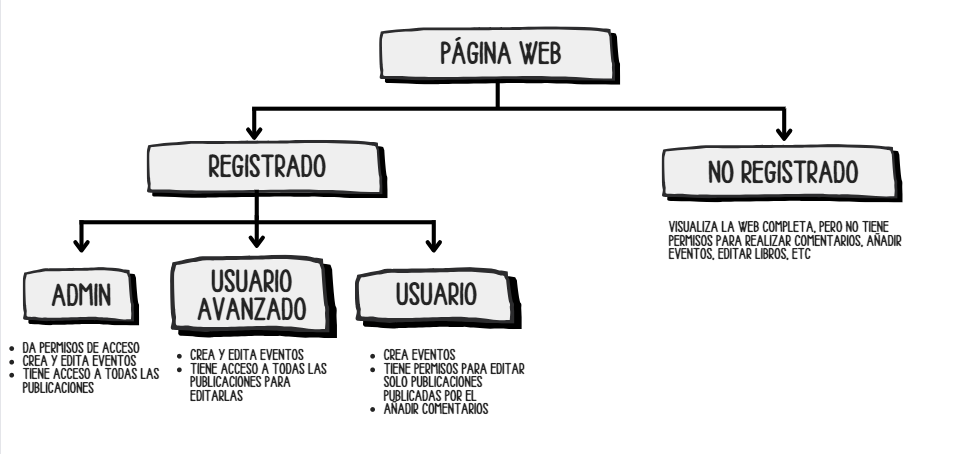
\includegraphics[width=9cm, keepaspectratio]{img/esquema.png}
  \caption{Estructura página web}
  \label{fig:arquitectura}
\end{figure}

\subsection{Vista de Usuario - No Registrado}
\label{sec:vista_usuarios_no_registrado}

\begin{itemize}
  \item \texttt{sitio/\_top\_of\_page.html}: Barra de navegación principal de la aplicación. Aquí se incluyen los enlaces a las diferentes páginas y funcionalidades del sitio web.
  \item \texttt{sitio/\_index.html}: Es la página de inicio de la plataforma.
  \item \texttt{sitio/\_books.html}: Se ocupa de la estructura y propiedades de la página de libros. Aquí es donde se muestran los libros en la plataforma y se pueden seleccionar para visualizar más detalles
  \item \textbf{}
    \begin{itemize}
        \item \texttt{/admin\_calendar()}: Muestra los eventos almacenados en la base de datos en un formato de calendario. Verifica los roles de los 
        usuarios para determinar si tienen permiso para acceder.
    \end{itemize}
\end{itemize}

\subsection{Vista de Usuario - Registrado}
\label{sec:vista_usuarios_registrado}

La pagina esta diseñada con el framework de Flask, utiliza una base de datos de xampp el cual esta
Por ejemplo, puedes verlo en la figura~\ref{fig:arquitectura}.
\LaTeX \ pone las figuras donde mejor cuadran. 
Y eso quiere decir que quizás no lo haga donde lo hemos puesto\ldots 
Eso no es malo.
A veces queda un poco raro, pero es la filosofía de \LaTeX: tú al contenido, que yo me encargo de la maquetación.


 
Recuerda que toda figura que añadas a tu memoria debe ser explicada.
Sí, aunque te parezca evidente lo que se ve en la figura~\ref{fig:arquitectura}, la figura en sí solamente es un apoyo a tu texto.
Así que explica lo que se ve en la figura, haciendo referencia a la misma tal y como ves aquí.
Por ejemplo: En la figura~\ref{fig:arquitectura} se puede ver que la estructura del \emph{parser} básico, que consta de seis componentes diferentes: los datos se obtienen de la red, y según el tipo de dato, se pasará a un \emph{parser} específico y bla, bla, bla\ldots

Si utilizas una base de datos, no te olvides de incluir también un diagrama de entidad-relación.



%%%%%%%%%%%%%%%%%%%%%%%%%%%%%%%%%%%%%%%%%%%%%%%%%%%%%%%%%%%%%%%%%%%%%%%%%%%%%%%%
%%%%%%%%%%%%%%%%%%%%%%%%%%%%%%%%%%%%%%%%%%%%%%%%%%%%%%%%%%%%%%%%%%%%%%%%%%%%%%%%
% EXPERIMENTOS Y VALIDACIÓN %
%%%%%%%%%%%%%%%%%%%%%%%%%%%%%%%%%%%%%%%%%%%%%%%%%%%%%%%%%%%%%%%%%%%%%%%%%%%%%%%%

\cleardoublepage
\chapter{Experimentos y validación}
\label{chap:experimentos}

Este capítulo se introdujo como requisito en 2019. 
Describe los experimentos y casos de test que tuviste que implementar para validar tus resultados. 
Incluye también los resultados de validación que permiten afirmar que tus resultados son correctos. 


%%%%%%%%%%%%%%%%%%%%%%%%%%%%%%%%%%%%%%%%%%%%%%%%%%%%%%%%%%%%%%%%%%%%%%%%%%%%%%%%
%%%%%%%%%%%%%%%%%%%%%%%%%%%%%%%%%%%%%%%%%%%%%%%%%%%%%%%%%%%%%%%%%%%%%%%%%%%%%%%%
% RESULTADOS %
%%%%%%%%%%%%%%%%%%%%%%%%%%%%%%%%%%%%%%%%%%%%%%%%%%%%%%%%%%%%%%%%%%%%%%%%%%%%%%%%

\cleardoublepage
\chapter{Resultados}
\label{chap:resultados}

En este capítulo se incluyen los resultados de tu trabajo fin de grado.

Si es una herramienta de análisis lo que has realizado, aquí puedes poner ejemplos de haberla utilizado para que se vea su utilidad.


%%%%%%%%%%%%%%%%%%%%%%%%%%%%%%%%%%%%%%%%%%%%%%%%%%%%%%%%%%%%%%%%%%%%%%%%%%%%%%%%
%%%%%%%%%%%%%%%%%%%%%%%%%%%%%%%%%%%%%%%%%%%%%%%%%%%%%%%%%%%%%%%%%%%%%%%%%%%%%%%%
% CONCLUSIONES %
%%%%%%%%%%%%%%%%%%%%%%%%%%%%%%%%%%%%%%%%%%%%%%%%%%%%%%%%%%%%%%%%%%%%%%%%%%%%%%%%

\cleardoublepage
\chapter{Conclusiones}
\label{chap:conclusiones}


\section{Consecución de objetivos}
\label{sec:consecucion-objetivos}

Esta sección es la sección espejo de las dos primeras del capítulo de objetivos, donde se planteaba el objetivo general y se elaboraban los específicos.

Es aquí donde hay que debatir qué se ha conseguido y qué no. 
Cuando algo no se ha conseguido, se ha de justificar, en términos de qué problemas se han encontrado y qué medidas se han tomado para mitigar esos problemas.

Y si has llegado hasta aquí, siempre es bueno pasarle el corrector ortográfico, que las erratas quedan fatal en la memoria final.
Para eso, en Linux tenemos aspell, que se ejecuta de la siguiente manera desde la línea de \emph{shell}:

\begin{verbatim}
  aspell --lang=es_ES -c memoria.tex
\end{verbatim}

\section{Aplicación de lo aprendido}
\label{sec:aplicacion}

Aquí viene lo que has aprendido durante el Grado/Máster y que has aplicado en el TFG/TFM.
Una buena idea es poner las asignaturas más relacionadas y comentar en un párrafo los conocimientos y habilidades puestos en práctica.

\begin{enumerate}
  \item a
  \item b
\end{enumerate}


\section{Lecciones aprendidas}
\label{sec:lecciones_aprendidas}

Aquí viene lo que has aprendido en el Trabajo Fin de Grado/Máster.

\begin{enumerate}
  \item Aquí viene uno.
  \item Aquí viene otro.
\end{enumerate}


\section{Trabajos futuros}
\label{sec:trabajos_futuros}

Ningún proyecto ni software se termina, así que aquí vienen ideas y funcionalidades que estaría bien tener implementadas en el futuro.

Es un apartado que sirve para dar ideas de cara a futuros TFGs/TFMs.


%%%%%%%%%%%%%%%%%%%%%%%%%%%%%%%%%%%%%%%%%%%%%%%%%%%%%%%%%%%%%%%%%%%%%%%%%%%%%%%%
%%%%%%%%%%%%%%%%%%%%%%%%%%%%%%%%%%%%%%%%%%%%%%%%%%%%%%%%%%%%%%%%%%%%%%%%%%%%%%%%
% APÉNDICE(S) %
%%%%%%%%%%%%%%%%%%%%%%%%%%%%%%%%%%%%%%%%%%%%%%%%%%%%%%%%%%%%%%%%%%%%%%%%%%%%%%%%

\cleardoublepage
\appendix
\chapter{Manual de usuario}
\label{app:manual}

Esto es un apéndice.
Si has creado una aplicación, siempre viene bien tener un manual de usuario.
Pues ponlo aquí.

%%%%%%%%%%%%%%%%%%%%%%%%%%%%%%%%%%%%%%%%%%%%%%%%%%%%%%%%%%%%%%%%%%%%%%%%%%%%%%%%
%%%%%%%%%%%%%%%%%%%%%%%%%%%%%%%%%%%%%%%%%%%%%%%%%%%%%%%%%%%%%%%%%%%%%%%%%%%%%%%%
% BIBLIOGRAFIA %
%%%%%%%%%%%%%%%%%%%%%%%%%%%%%%%%%%%%%%%%%%%%%%%%%%%%%%%%%%%%%%%%%%%%%%%%%%%%%%%%

\cleardoublepage

% Las siguientes dos instrucciones es todo lo que necesitas
% para incluir las citas en la memoria
\bibliographystyle{abbrv}
\bibliography{memoria}  % memoria.bib es el nombre del fichero que contiene
% las referencias bibliográficas. Abre ese fichero y mira el formato que tiene,
% que se conoce como BibTeX. Hay muchos sitios que exportan referencias en
% formato BibTeX. Prueba a buscar en http://scholar.google.com por referencias
% y verás que lo puedes hacer de manera sencilla.
% Más información: 
% http://texblog.org/2014/04/22/using-google-scholar-to-download-bibtex-citations/

\end{document}
